\documentclass[tikz,border=12pt]{standalone}
\usepackage{amsmath,amssymb}
\usepackage{tikz}
\usetikzlibrary{arrows.meta,positioning,fit,calc,backgrounds}
\tikzset{
  box/.style={
    draw,
    very thick,
    rectangle,
    align=center,
    inner sep=8pt,
    minimum height=1.25cm,
    minimum width=3.1cm,
    font=\small,
  },
  wide/.style={box, minimum width=3.6cm},
  arr/.style={-{Stealth[length=2.6mm, width=2mm]}, thick},
  barr/.style={
    {Stealth[length=2.4mm, width=1.8mm]}-{Stealth[length=2.4mm, width=1.8mm]},
    thick,
  },
  lbl/.style={font=\scriptsize, inner sep=2pt, fill=white},
  group/.style={draw, dashed, inner sep=12pt},
}

\begin{document}
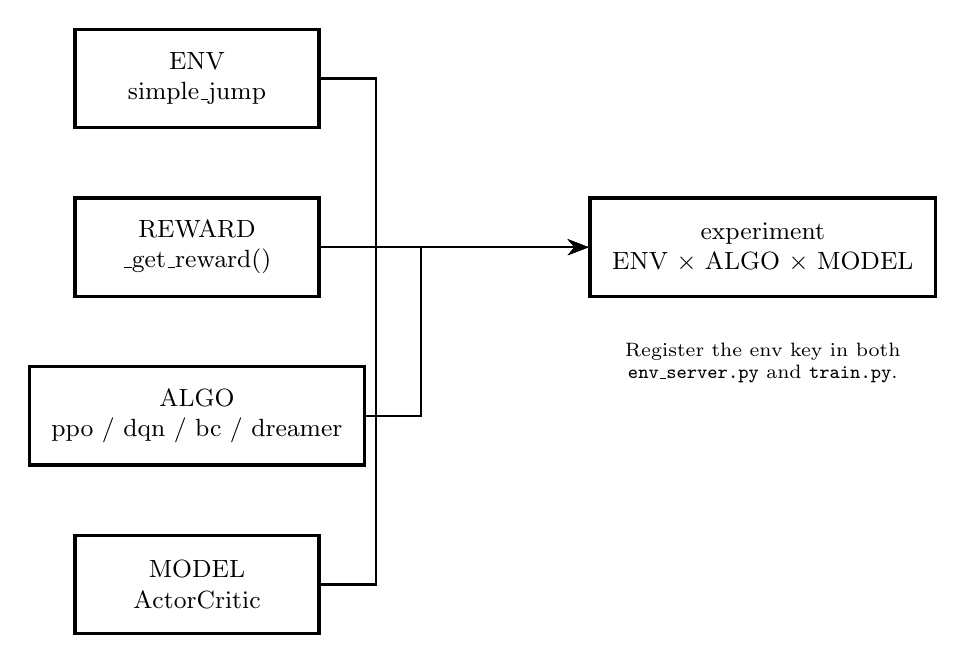
\begin{tikzpicture}[node distance=0.85cm and 1.1cm]
  \node[box] (env) {ENV\\simple\_jump};
  \node[box, below=of env] (rew) {REWARD\\\_get\_reward()};
  \node[box, below=of rew] (alg) {ALGO\\ppo / dqn / bc / dreamer};
  \node[box, below=of alg] (mod) {MODEL\\ActorCritic};

  \node[wide, right=3.4cm of rew] (exp) {experiment\\ENV $\times$ ALGO $\times$ MODEL};

  \draw[arr] (env.east) -- ++(0.7,0) |- (exp.west);
  \draw[arr] (rew) -- (exp);
  \draw[arr] (alg.east) -- ++(0.7,0) |- (exp.west);
  \draw[arr] (mod.east) -- ++(0.7,0) |- (exp.west);

  \node[font=\scriptsize, below=0.45cm of exp, text width=4.2cm, align=center] {%
    Register the env key in both \texttt{env\_server.py} and \texttt{train.py}.};
\end{tikzpicture}
\end{document}
